\section{Pass/Fail Plots}\label{app:tables}

The full set of constraint results for the fiducial models is presented below in graphical form.
In each plot the green models pass the constraint or constraints for \kharma, \bhac, and \hamr version of the model, while the red models fail the constraint or constraints for \kharma, \bhac, and \hamr.
The yellow models have different results for the different codes.
Notice that \hamr models are available only for $i = 10, 50, 90$deg; at $30, 70$deg only the \kharma and \bhac models are compared.

% First the EHT constraints.

\begin{figure*}
  \centering
  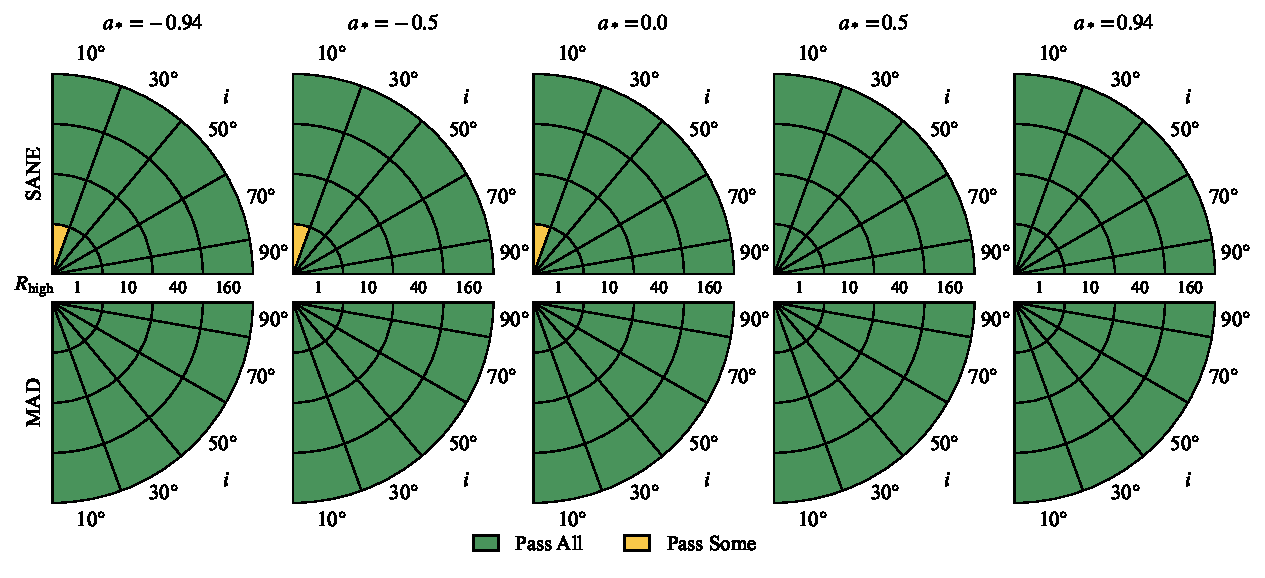
\includegraphics[width=0.8\textwidth]{./figures/230GHz_size_Constraints.pdf}
  \caption{2nd Moment Constraint.  Green indicates that the \kharma, \bhac, and \hamr models pass, yellow that one or two of the fiducial models fail, and red that all three fail.}
  \label{fig:230GHz_size_pizza}
\end{figure*}

\begin{figure*}
  \centering
  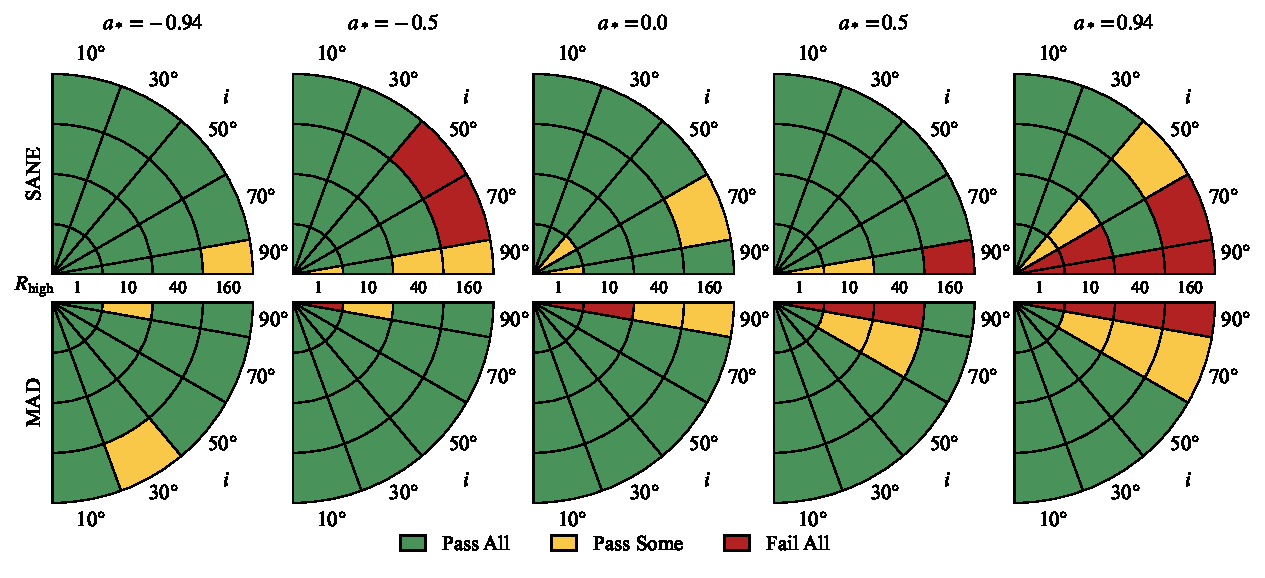
\includegraphics[width=0.8\textwidth]{./figures/Null_loc_Constraints.pdf}
  \caption{Null Location Constraint.  Green indicates that the \kharma, \bhac, and \hamr models pass, yellow that one or two of the fiducial models fail, and red that all three fail.}
  \label{fig:null_pizza}
\end{figure*}

\begin{figure*}
  \centering
  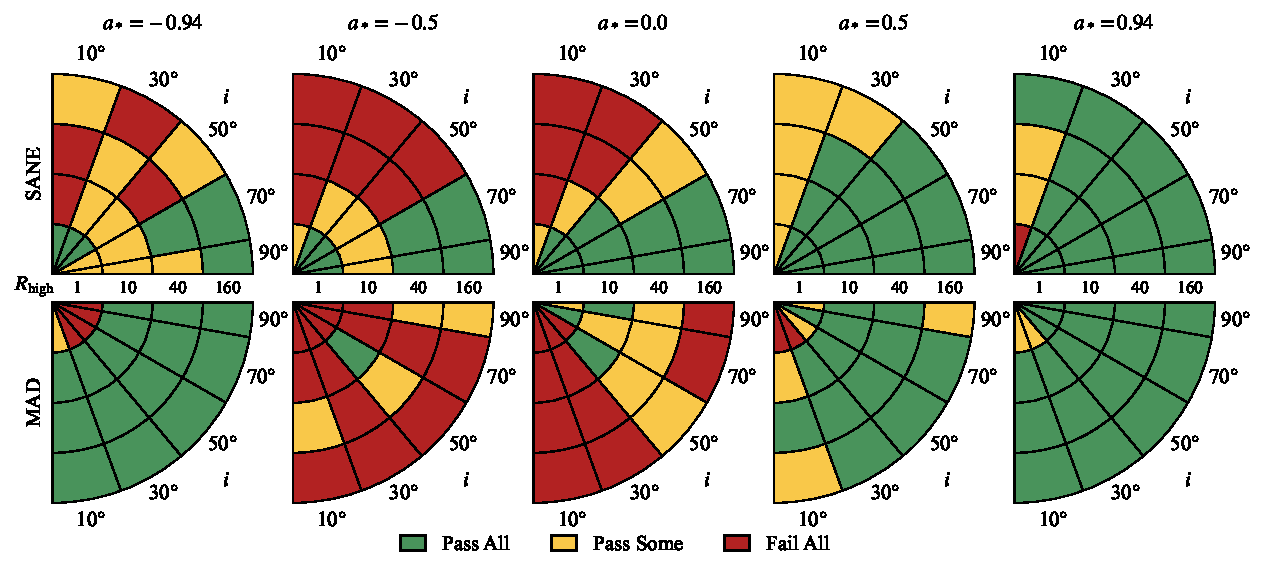
\includegraphics[width=0.8\textwidth]{./figures/Mring_d_Constraints.pdf}
  \caption{M-ring Diameter Constraints.  Green indicates that the \kharma, \bhac, and \hamr models pass, yellow that one or two of the fiducial models fail, and red that all three fail.}
  \label{fig:mring_diam_pizza}
\end{figure*}

\begin{figure*}
  \centering
  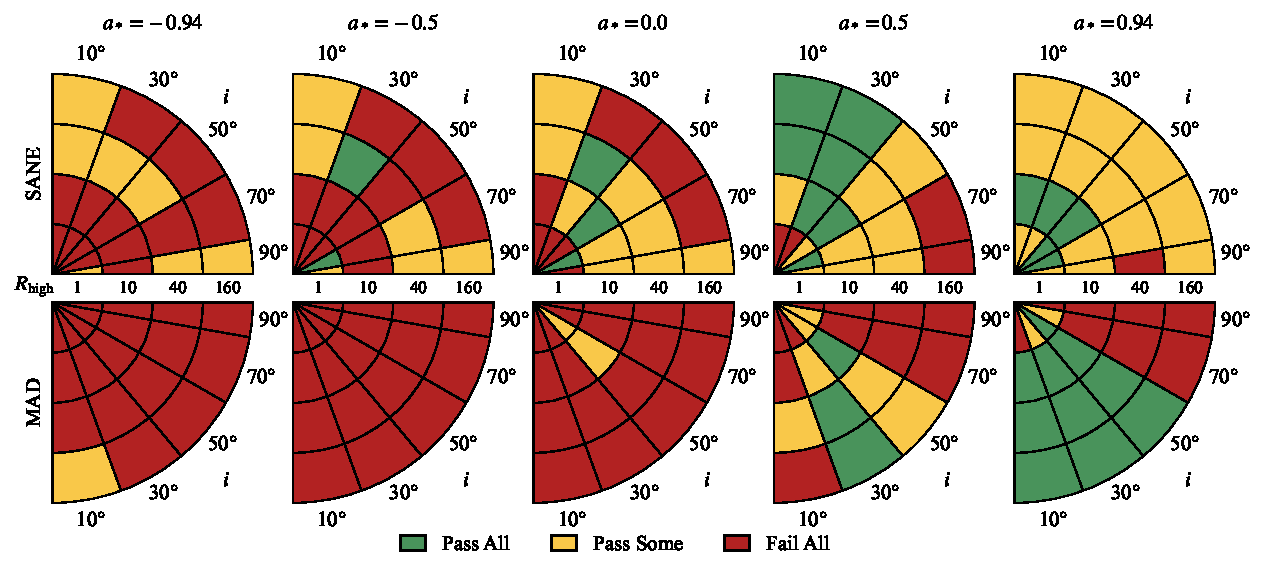
\includegraphics[width=0.8\textwidth]{./figures/Mring_w_Constraints.pdf}
  \caption{M-ring Width Constraints.  Green indicates that the \kharma, \bhac, and \hamr models pass, yellow that one or two of the fiducial models fail, and red that all three fail.}
  \label{fig:mring_width_pizza}
\end{figure*}

\begin{figure*}
  \centering
  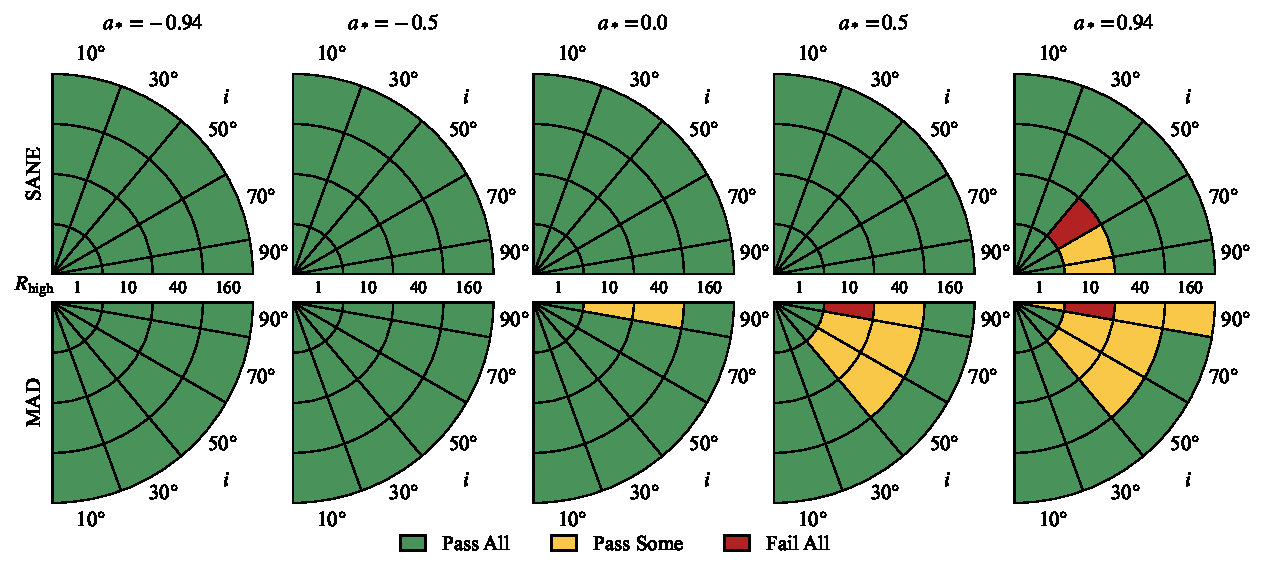
\includegraphics[width=0.8\textwidth]{./figures/Mring_f1_Constraints.pdf}
  \caption{M-ring Asymmetry Constraints.  Green indicates that the \kharma, \bhac, and \hamr models pass, yellow that one or two of the fiducial models fail, and red that all three fail.}
  \label{fig:mring_asymm_pizza}
\end{figure*}

\begin{figure*}
  \centering
  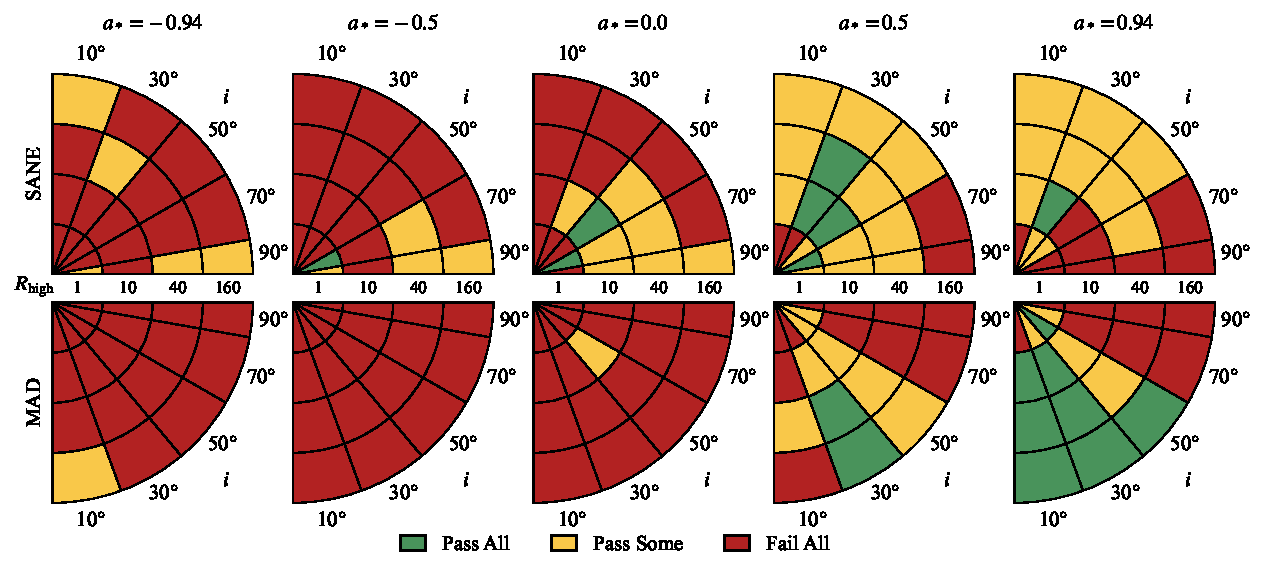
\includegraphics[width=0.8\textwidth]{./figures/Interferometric_Constraints.pdf}
  \caption{Combined EHT Constraints.  Green indicates that the \kharma, \bhac, and \hamr models pass, yellow that one or two of the fiducial models fail, and red that all three fail.}
  \label{fig:eht_comb_pizza}
\end{figure*}

%Then the non-EHT constraints.

\begin{figure*}
  \centering
  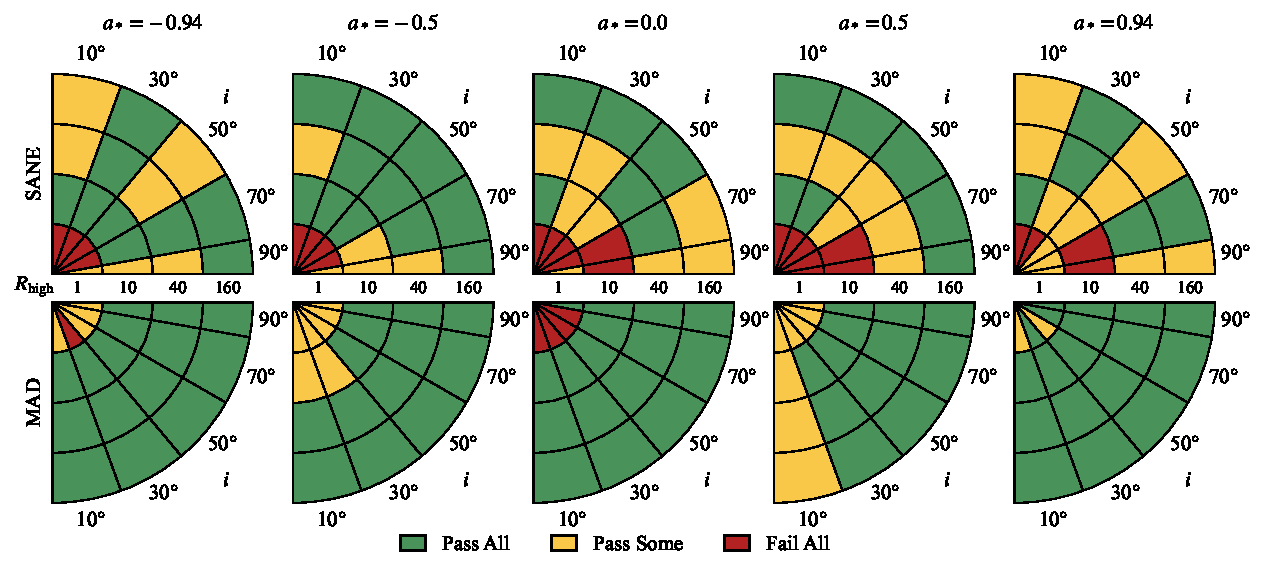
\includegraphics[width=0.8\textwidth]{./figures/86GHz_flux_Constraints.pdf}
  \caption{86GHz Flux Constraints.  Green indicates that the \kharma, \bhac, and \hamr models pass, yellow that one or two of the fiducial models fail, and red that all three fail.}
  \label{fig:86GHz_flux_pizza}
\end{figure*}

\begin{figure*}
  \centering
  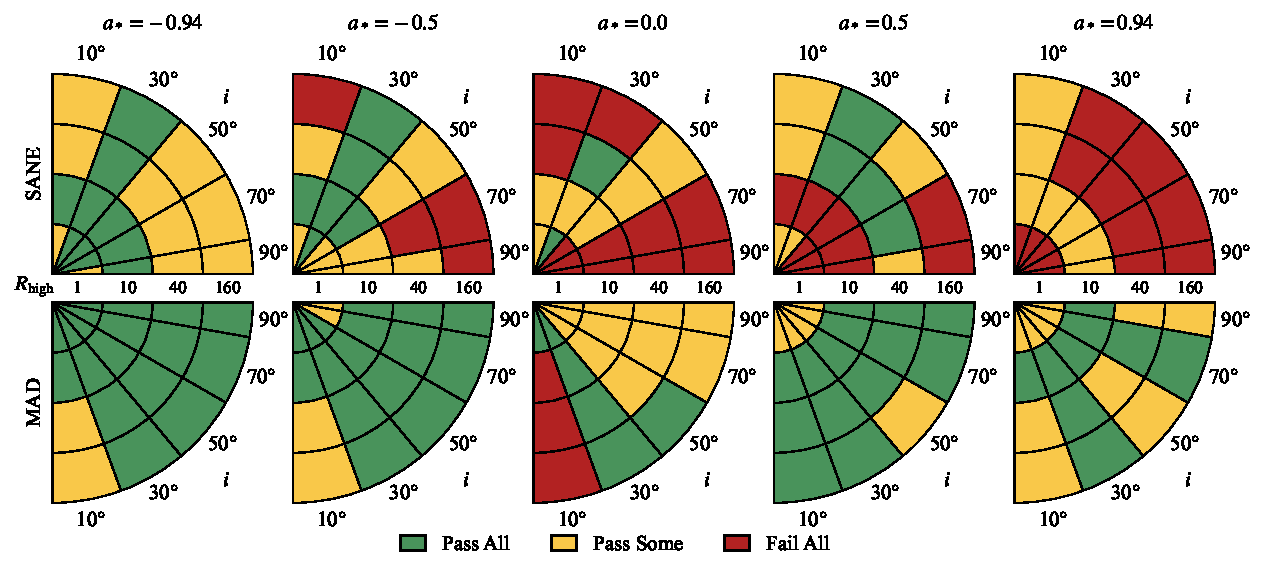
\includegraphics[width=0.8\textwidth]{./figures/86GHz_size_Constraints.pdf}
  \caption{86GHz Size Constraints.  Green indicates that the \kharma, \bhac, and \hamr models pass, yellow that one or two of the fiducial models fail, and red that all three fail.}
  \label{fig:86GHz_size_pizza}
\end{figure*}

\begin{figure*}
  \centering
  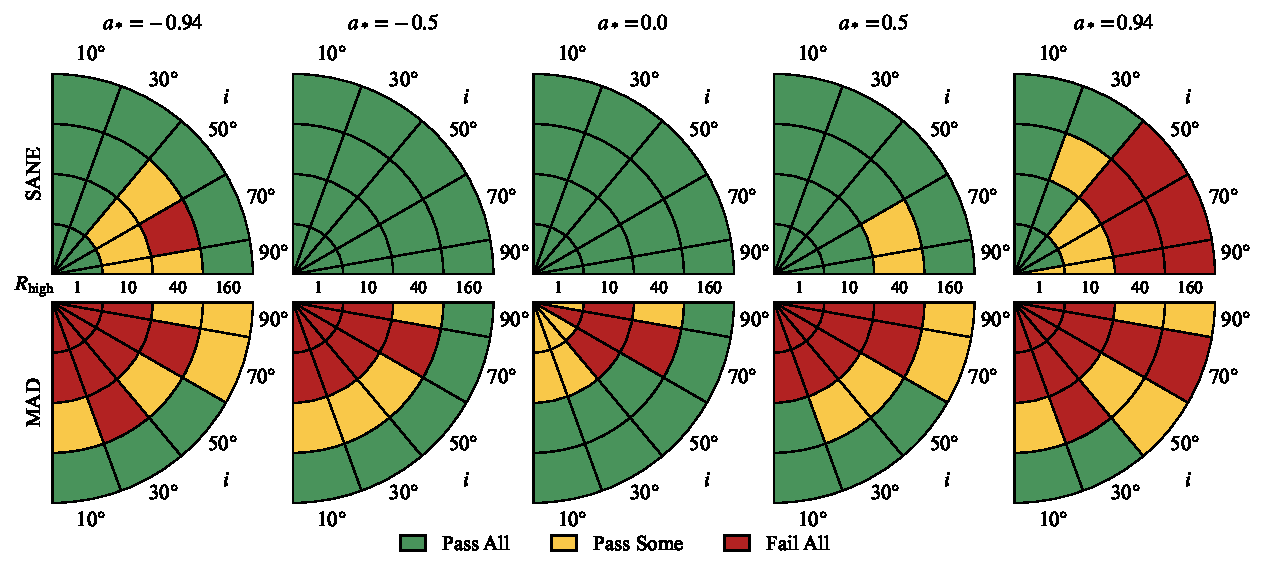
\includegraphics[width=0.8\textwidth]{./figures/2um_flux_Constraints.pdf}
  \caption{$2.2\mu$m Flux Constraints.  Green indicates that the \kharma, \bhac, and \hamr models pass, yellow that one or two of the fiducial models fail, and red that all three fail.}
  \label{fig:2um_flux_pizza}
\end{figure*}

\begin{figure*}
  \centering
  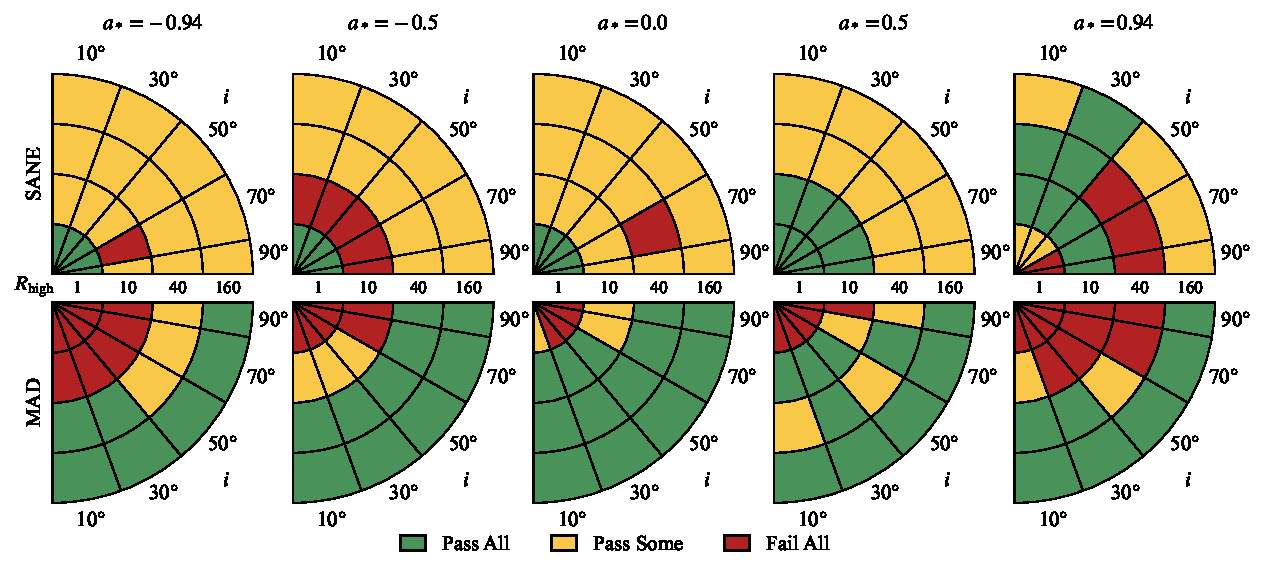
\includegraphics[width=0.8\textwidth]{./figures/Xray_flux_Constraints.pdf}
  \caption{X-Ray Luminosity Constraints.  Green indicates that the \kharma, \bhac, and \hamr models pass, yellow that one or two of the fiducial models fail, and red that all three fail.}
  \label{fig:xray_pizza}
\end{figure*}

\begin{figure*}
  \centering
  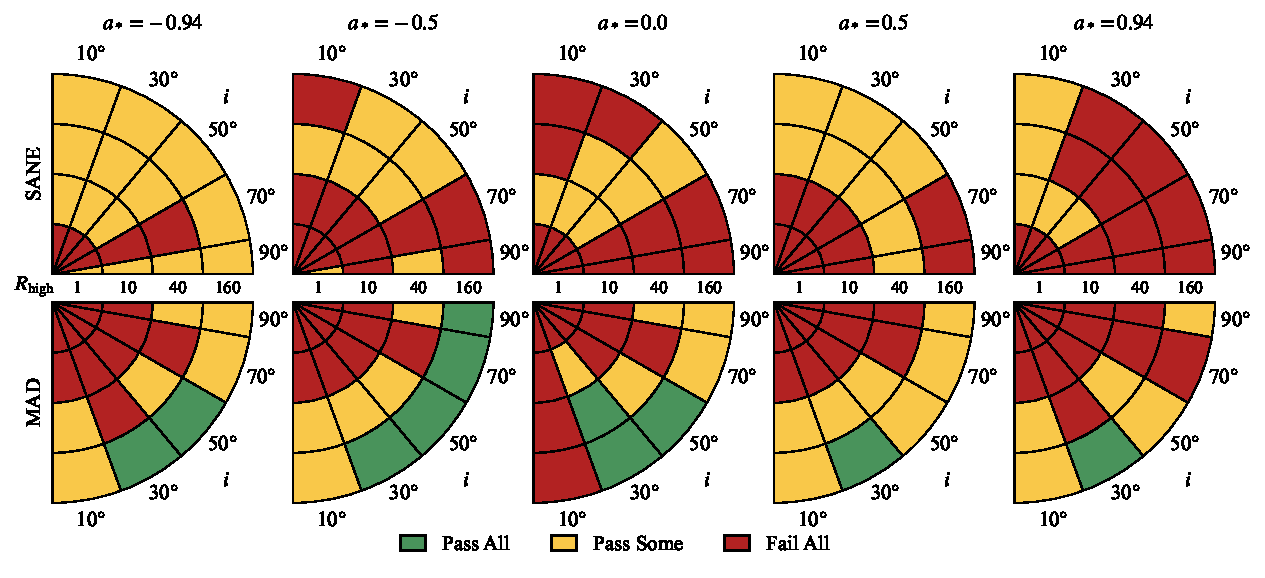
\includegraphics[width=0.8\textwidth]{./figures/Non_Interferometric_Constraints.pdf}
  \caption{Combined non-EHT Constraints.  Green indicates that the \kharma, \bhac, and \hamr models pass, yellow that one or two of the fiducial models fail, and red that all three fail.}
  \label{fig:noneht_pizza}
\end{figure*}

%Then the full set of combined constraints, without variability.

\begin{figure*}
  \centering
  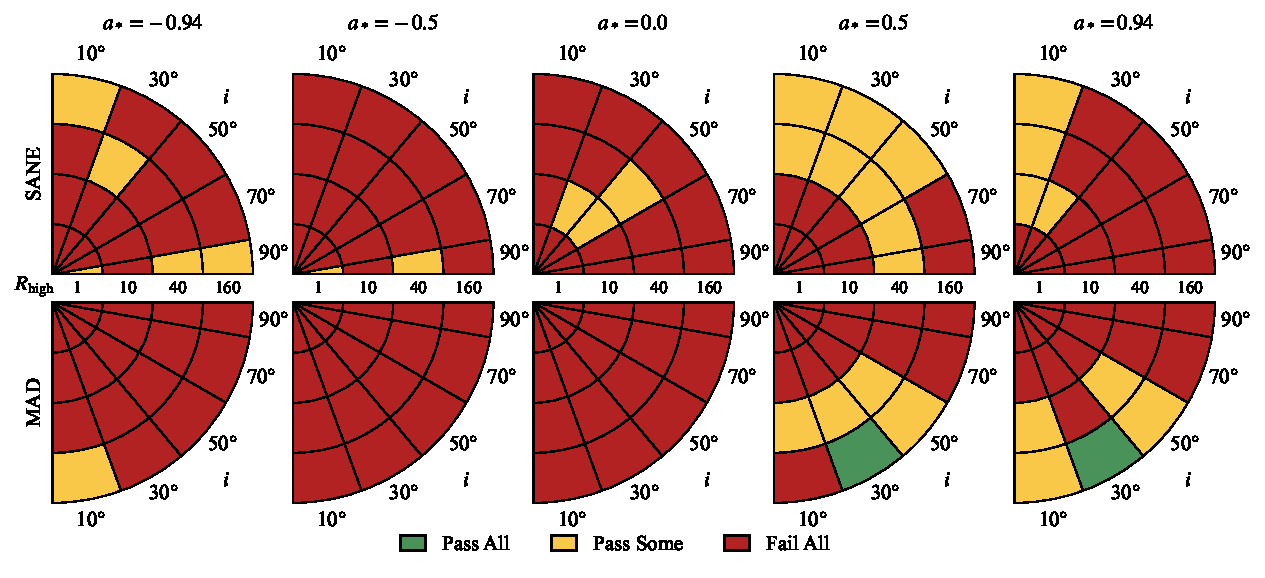
\includegraphics[width=0.8\textwidth]{./figures/All_Constraints.pdf}
  \caption{Combined constraints without structural or flux variability.  Green indicates that the \kharma, \bhac, and \hamr models pass, yellow that one or two of the fiducial models fail, and red that all three fail.}
  \label{fig:all_pizza_app}
\end{figure*}

%Then the variability constraints.

\begin{figure*}
  \centering
  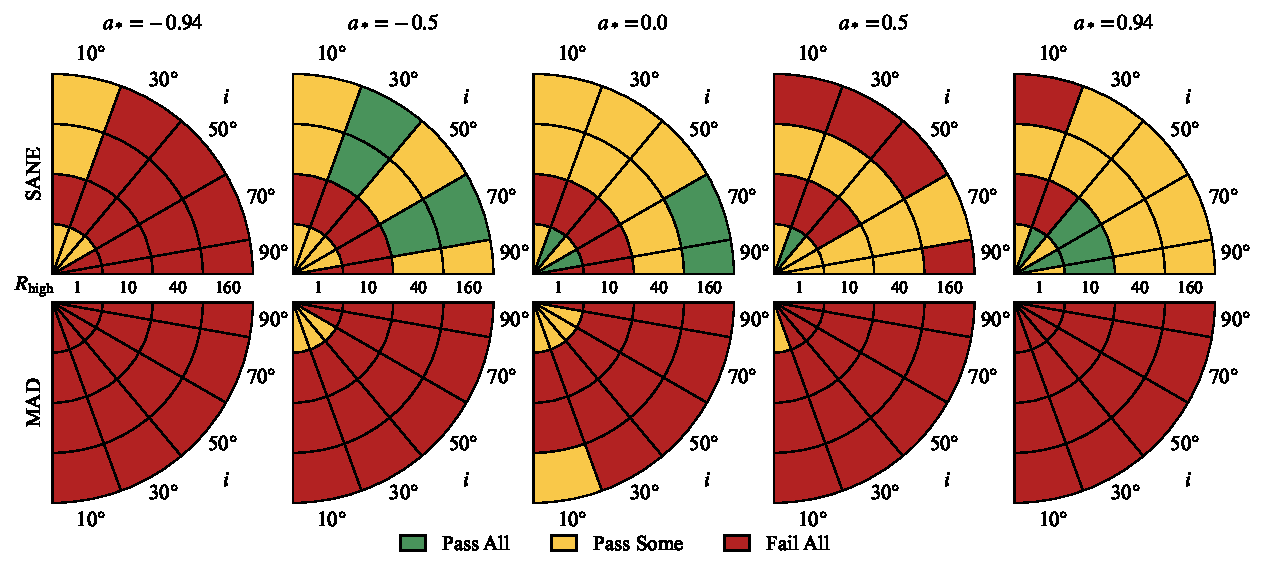
\includegraphics[width=0.8\textwidth]{./figures/230GHz_3Hr_MI_Constraints.pdf}
  \caption{$M_3$ Constraints.  Green indicates that the \kharma, \bhac, and \hamr models pass, yellow that one or two of the fiducial models fail, and red that all three fail.}
  \label{fig:m3_pizza}
\end{figure*}

\begin{figure*}
  \centering
  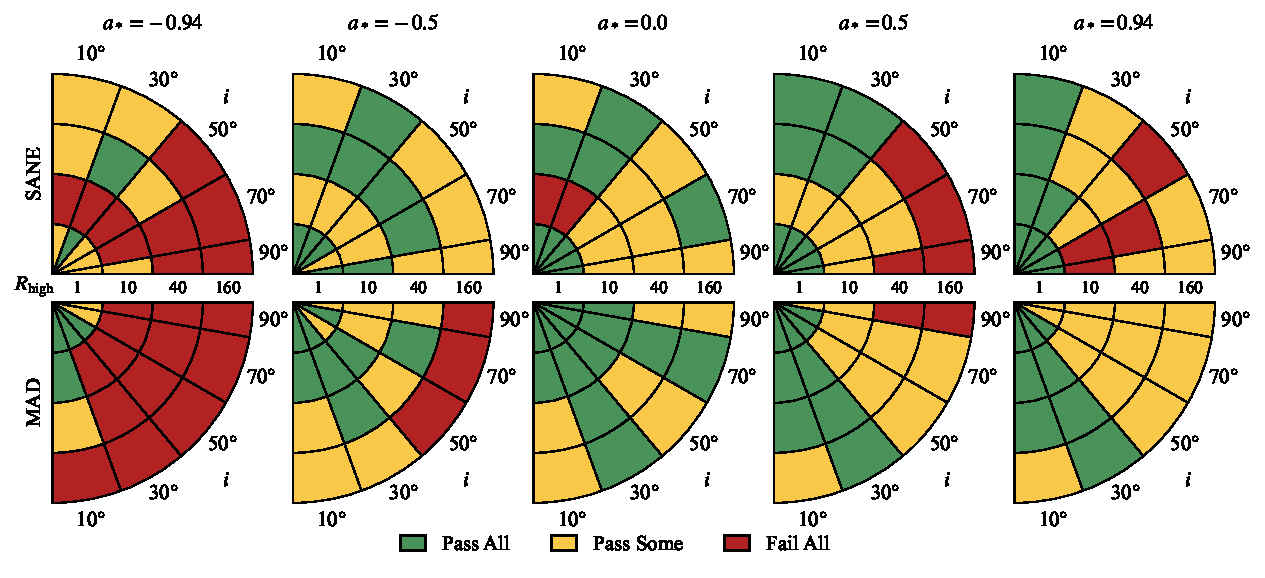
\includegraphics[width=0.8\textwidth]{./figures/4Glam_Constraints.pdf}
  \caption{EHT Structural Variability Constraints.  Green indicates that the \kharma, \bhac, and \hamr models pass, yellow that one or two of the fiducial models fail, and red that all three fail.}
  \label{fig:ehtvar_pizza}
\end{figure*}

\clearpage
